\section{Structural and practical parameter identifiability}
\label{sec:identifiability}
The observations in Eq.~\eqref{main-eq:binned_observation} of the main article are two activity series, not direct measurements of the seven human compartments or either media state. We therefore examine the observation map before interpreting any inverse estimate. A product in one transition rate does not by itself prove that its factors are unidentifiable: those factors may enter other equations differently. Here, non-identifiability follows from an explicit symmetry of the complete delay model.

\begin{theorem}[Unidentifiable media scale]
\label{thm:media_scale}
Suppose the media scale, its history, and its associated coefficients are unknown. For any $c>0$, define
\begin{equation}
\begin{aligned}
\widetilde M_i&=cM_i,\quad\widetilde\chi=c\chi,\quad\widetilde\rho=\rho/c^2,\\
(\widetilde\varpi_i,\widetilde\kappa_i,\widetilde\delta_i)
  &=(\varpi_i,\kappa_i,\delta_i)/c,\\
(\widetilde q_R,\widetilde q_D)&=(q_R,q_D)/c,\\
(\widetilde\eta_i,\widetilde v_i)&=c(\eta_i,v_i),
\end{aligned}
\label{eq:media_symmetry}
\end{equation}
for $i=1,2$, with media history multiplied by $c$. Leave the human states, their history, $\tau$, $q_U$, decay rates, and reporting scales unchanged. These distinct parameter vectors generate identical observations. Thus the unrestricted inverse problem is structurally non-identifiable.
\end{theorem}
\begin{proof}
The transformation leaves $\rho M_1M_2$, $\varpi_iM_i$, $\kappa_iM_i$, $\delta_iM_i$, $q_RM_2$, and $q_DM_1$ unchanged. It also preserves $\chi/(\chi+M_1+M_2)$ and $\Gamma_U$. Hence $p$, all three $\Gamma$ rates, the incidence, and $Q_\tau$ are unchanged at both current and delayed times. Each human equation is identical, whereas each media equation and its left-hand side are multiplied by $c$. Both entry fluxes and their bin integrals are consequently identical. The same transformation preserves the history-compatibility inequality. This constructs a continuous family of indistinguishable solutions, including arbitrarily close parameter vectors.
\end{proof}

Writing $m_i=M_i/\chi$ exposes invariant combinations such as $q_R\chi$, $q_D\chi$, $\varpi_i\chi$, $\kappa_i\chi$, $\delta_i\chi$, $\rho\chi^2$, $\eta_i/\chi$, and $v_i/\chi$. These combinations remove this scale ambiguity; their individual identifiability does not follow automatically. Finding one symmetry proves non-identifiability, but removing it does not exclude other symmetries~\cite{villaverde2021scaling}. Our symbolic audit verifies all nine transformed state equations, both observation fluxes, and the intermediate rate identities exactly.

\subsection{Conditional estimation and complete parameter specification}
Table~\ref{tab:empirical_parameters} specifies every fixed value, estimated range, and initialization used in the empirical code. Fixed values are modeling assumptions, not independent measurements or fitted values with zero uncertainty. The common media history and fixed media coefficients choose a scale and remove the family in Theorem~\ref{thm:media_scale}. Only
\[
\vartheta=(\beta_1,\beta_2,\tau_s,q_R,q_D,\chi,
\widetilde s_R,\widetilde s_D)
\]
is adjusted. The last two quantities are the implementation's reporting gains after bin width and training-count normalization are absorbed. All rates in this table use normalized time: for a fold of duration $T_e$ hours, $k_{\rm hourly}=k_{\rm normalized}/T_e$ and $\tau_{\rm hours}=T_e\tau_s$. No Bayesian priors are used. Table~\ref{tab:neural_parameters} reports the actual validation-selected neural estimates across all four events; its fold ranges describe variability, not confidence intervals.

\begin{table*}[t]
\centering\scriptsize
\caption{Complete empirical parameter specification. Time unit $\mathsf T$ denotes one normalized event horizon; media indices and human proportions are dimensionless. Bounds are hard constraints, not priors. Fixed quantities have no fitted uncertainty interval. Estimated values are reported in Tables~\ref{tab:neural_parameters} and~\ref{tab:profile_parameters}.}
\label{tab:empirical_parameters}
\begin{tabular}{lllll}
\toprule Quantity & Role & Normalized unit & Fixed value or allowed range & Neural initialization\\\midrule
$\beta_1$ & estimated exposure rate & $\mathsf T^{-1}$ & $[0.10,8.00]$ & 2.4700\\
$\beta_2$ & estimated exposure rate & $\mathsf T^{-1}$ & $[0.05,5.00]$ & 1.2875\\
$\tau_s$ & estimated processing delay & $\mathsf T$ & $[0.01,0.22]$ & 0.0730\\
$q_R,q_D$ & estimated adoption coefficients & $\mathsf T^{-1}$ & each $[0.05,4.00]$ & each 1.0375\\
$\chi$ & estimated fatigue threshold & 1 & $[0.05,3.00]$ & 1.0825\\
$\widetilde s_R,\widetilde s_D$ & estimated normalized reporting gains & 1 & each $[0.25,12.00]$ & each 0.8375\\\midrule
$\Lambda,d_h$ & closed-event recruitment and exit & $\mathsf T^{-1}$ & both 0 & fixed\\
$\lambda$ & recruitment allocation & 1 & inactive because $\Lambda=0$ & not fitted\\
$N$ & human population normalization & 1 & 1 & fixed\\
$\varepsilon$ & relative exposure susceptibility & 1 & 0.55 & fixed\\
$\kappa_1,\kappa_2$ & media-driven susceptibility transitions & $\mathsf T^{-1}$ & 0.40, 0.25 & fixed\\
$\xi_E,\sigma_E,\gamma_E$ & direct exits from exposure & $\mathsf T^{-1}$ & 0.80, 0.40, 0.20 & fixed\\
$a_E$ & total competing exit rate & $\mathsf T^{-1}$ & 1.40 (derived) & not fitted\\
$\rho$ & cohort-pathway gate coefficient & 1 & 5.00 & fixed\\
$\mu,\alpha$ & withdrawal rates & $\mathsf T^{-1}$ & both 0.25 & fixed\\
$\delta_1,\delta_2$ & media-driven $R/D$ conversion & $\mathsf T^{-1}$ & 0.50, 0.25 & fixed\\
$\eta_1,\eta_2$ & media generation & $\mathsf T^{-1}$ & both 0.60 & fixed\\
$v_1,v_2$ & external media input & $\mathsf T^{-1}$ & both 0.20 & fixed\\
$d_{M_1},d_{M_2}$ & media decay & $\mathsf T^{-1}$ & both 1.00 & fixed\\
$\varpi_1,\varpi_2$ & cross-media inhibition & 1 & both 1.00 & fixed\\
$q_U$ & fatigue withdrawal coefficient & $\mathsf T^{-1}$ & 0.30 & fixed\\
$\phi_{S_u,S_e,E,H,R,D,U}$ & constant human history on $[-\tau_s,0]$ & 1 & $(.93,.03,.015,.005,.010,.005,.005)$ & fixed\\
$\phi_{M_1,M_2}$ & constant media history on $[-\tau_s,0]$ & 1 & $(.20,.20)$ & fixed\\
\bottomrule
\end{tabular}
\end{table*}

\begin{table*}[t]
\centering\scriptsize
\caption{Validation-selected TransPINN parameter values: median [minimum, maximum] over the three rolling folds of each event. These describe the fitted neural coefficients in the forecasting experiment, not physical parameter confidence intervals. All 12 vectors and all eight quantities are archived.}
\label{tab:neural_parameters}
\setlength{\tabcolsep}{7pt}
\begin{tabular}{lcccc}
\toprule Parameter & Harvey & CSDC & Ottawa & Sydney\\\midrule
$\beta_1$ & $2.2594\;[2.1396,\,2.3054]$ & $2.1374\;[2.0175,\,2.3465]$ & $2.0614\;[2.0538,\,2.3875]$ & $2.3314\;[2.0346,\,2.4184]$ \\
$\beta_2$ & $1.1689\;[1.0954,\,1.2114]$ & $1.1070\;[1.0303,\,1.2230]$ & $1.0603\;[1.0531,\,1.2415]$ & $1.2103\;[1.0538,\,1.2608]$ \\
$\tau_s$ & $0.0684\;[0.0666,\,0.0736]$ & $0.0742\;[0.0726,\,0.0746]$ & $0.0695\;[0.0691,\,0.0726]$ & $0.0727\;[0.0716,\,0.0732]$ \\
$q_R$ & $0.9906\;[0.9900,\,0.9948]$ & $1.0041\;[1.0009,\,1.0213]$ & $1.1419\;[1.0110,\,1.1725]$ & $1.0056\;[1.0026,\,1.0144]$ \\
$q_D$ & $0.9932\;[0.9887,\,0.9979]$ & $1.0667\;[1.0198,\,1.1117]$ & $1.1551\;[1.0171,\,1.1706]$ & $1.0075\;[1.0065,\,1.1028]$ \\
$\chi$ & $1.0461\;[1.0384,\,1.0531]$ & $1.0844\;[1.0795,\,1.0894]$ & $1.1882\;[1.0697,\,1.2012]$ & $1.0752\;[1.0586,\,1.1116]$ \\
$\widetilde s_R$ & $0.8263\;[0.8257,\,0.8291]$ & $0.8492\;[0.8474,\,0.8501]$ & $0.8474\;[0.8467,\,0.8484]$ & $0.8437\;[0.8430,\,0.8437]$ \\
$\widetilde s_D$ & $0.8251\;[0.8250,\,0.8294]$ & $0.8439\;[0.8418,\,0.8452]$ & $0.8440\;[0.8428,\,0.8455]$ & $0.8444\;[0.8400,\,0.8451]$ \\
\\[-6pt]\bottomrule
\end{tabular}
\end{table*}


\subsection{Local sensitivity of the DDE observation map}
We integrate the DDE independently of the neural network and form the training-only elasticity matrix
\begin{equation}
S_{(j,k),\ell}=\frac{\partial\log g_k(s_j;\vartheta)}
 {\partial\log\vartheta_\ell},\qquad k\in\{R,D\},
\label{eq:ident_sensitivity}
\end{equation}
where $g$ uses the same right-endpoint observation convention as the empirical solver. Central log-parameter perturbations of $10^{-3}$ are applied at each of the 12 validation-selected event--fold parameter vectors. At relative singular-value cutoff $10^{-6}$, all 12 matrices have rank eight. However, their condition numbers range from $2.38\times10^5$ to $4.93\times10^5$; only four or five singular directions exceed $10^{-3}$ of the largest singular value. Halving the perturbation and integration step changes the sensitivity matrix by less than $1.5\times10^{-7}$ in relative Frobenius norm. The full rank is therefore numerically reproducible but coexists with strong practical confounding. It is a local diagnostic under fixed history and nuisance coefficients, not a proof of global structural identifiability.

\begin{figure}[t]
\centering
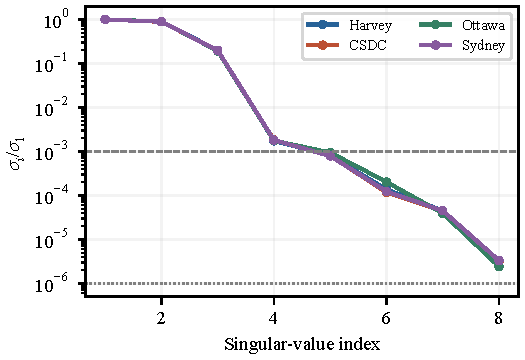
\includegraphics[width=.98\columnwidth]{output/identifiability/sensitivity_spectrum.pdf}
\caption{Training-only sensitivity spectra for the prespecified middle fold. All eight singular values exceed the $10^{-6}$ relative cutoff, but several directions are weak. Dashed and dotted lines mark $10^{-3}$ and $10^{-6}$.}
\label{fig:ident_spectrum}
\end{figure}

\subsection{Profile likelihood and parameter uncertainty}
A neural parameter estimate is not automatically a likelihood estimate for the DDE. We therefore fit the independently integrated model to the training block of the prespecified middle fold of each event. Only training observations enter the likelihood. These four diagnostic fits are separate from the forecasting benchmark. With $A_k$ the training total, $d_k=\max\{1,\operatorname{RMS}(Y_{k,\mathrm{train}})\}$, and $n=2n_{\rm tr}$, define
\begin{equation}
\operatorname{RSS}(\vartheta)=\sum_{j,k}
\left[\frac{g_k(s_j;\vartheta)-Y_{k,j}/A_k}{d_k/A_k}\right]^2.
\label{eq:ident_rss}
\end{equation}
We use a working Gaussian error model with a common unknown variance for these standardized residuals. Six starting points are optimized within the declared bounds: the archived neural estimate, the geometric midpoint of the bounds, and four log-uniform draws with seed 20260918. For each parameter value $a$, all seven remaining parameters are re-optimized, giving $\operatorname{RSS}_{\ell}(a)$. Following the profile-likelihood approach~\cite{raue2009identifiability}, the nominal 95\% support interval containing the best fit satisfies
\begin{equation}
n\log\!\left[\frac{\operatorname{RSS}_{\ell}(a)}
 {\operatorname{RSS}(\widehat\vartheta)}\right]\leq3.841.
\label{eq:ident_profile}
\end{equation}
We evaluate 17 log-spaced values plus the optimum, use two nuisance-parameter starts at each value, and refine threshold crossings numerically. A fixed RK4 method of steps uses spacing $1/4000$ and linear interpolation of past states. Step refinement and an independent adaptive integrator check the observation map. These are conditional, pointwise, asymptotic intervals. They are not neural prediction bands or Bayesian credible intervals. Their coverage is not calibrated for serial dependence, sparse counts, or boundary estimates.

\begin{table*}[t]
\centering\scriptsize
\caption{Independent DDE diagnostic estimates and nominal 95\% profile support intervals, using training data from fold 2 only. All values use the normalized units in Table~\ref{tab:empirical_parameters}. An asterisk marks an endpoint imposed by the search bound because no likelihood crossing was found. An interval spanning both bounds is not evidence that the parameter is well determined. These intervals belong to the DDE fits, not the neural estimates in Table~\ref{tab:neural_parameters}.}
\label{tab:profile_parameters}
\setlength{\tabcolsep}{5pt}
\begin{tabular}{lcccc}
\toprule Parameter & Harvey & CSDC & Ottawa & Sydney\\\midrule
$\beta_1$ & $2.882\;[1.805,\,6.562]$ & $2.517\;[0.100^{*},\,8.000^{*}]$ & $0.100\;[0.100^{*},\,0.712]$ & $0.100\;[0.100^{*},\,0.344]$ \\
$\beta_2$ & $5.000\;[0.050^{*},\,5.000^{*}]$ & $0.050\;[0.050^{*},\,5.000^{*}]$ & $0.050\;[0.050^{*},\,1.162]$ & $0.050\;[0.050^{*},\,0.500]$ \\
$\tau_s$ & $0.010\;[0.010^{*},\,0.220^{*}]$ & $0.220\;[0.010^{*},\,0.220^{*}]$ & $0.010\;[0.010^{*},\,0.220^{*}]$ & $0.010\;[0.010^{*},\,0.220^{*}]$ \\
$q_R$ & $0.050\;[0.050^{*},\,4.000^{*}]$ & $0.648\;[0.050^{*},\,4.000^{*}]$ & $0.050\;[0.050^{*},\,4.000^{*}]$ & $0.050\;[0.050^{*},\,4.000^{*}]$ \\
$q_D$ & $1.636\;[0.050^{*},\,4.000^{*}]$ & $4.000\;[0.050^{*},\,4.000^{*}]$ & $2.680\;[0.050^{*},\,4.000^{*}]$ & $0.050\;[0.050^{*},\,4.000^{*}]$ \\
$\chi$ & $3.000\;[0.050^{*},\,3.000^{*}]$ & $3.000\;[0.050^{*},\,3.000^{*}]$ & $0.367\;[0.050^{*},\,3.000^{*}]$ & $0.050\;[0.050^{*},\,3.000^{*}]$ \\
$\widetilde s_R$ & $0.250\;[0.250^{*},\,0.267]$ & $2.324\;[0.341,\,5.162]$ & $5.195\;[3.163,\,6.450]$ & $3.041\;[1.843,\,3.770]$ \\
$\widetilde s_D$ & $0.390\;[0.276,\,0.546]$ & $2.750\;[0.967,\,7.063]$ & $6.490\;[3.856,\,9.712]$ & $4.789\;[2.489,\,6.108]$ \\
\\[-6pt]\bottomrule
\end{tabular}
\end{table*}

The profile curves are shown in Fig.~\ref{main-fig:ident_profiles} of the main article.

Table~\ref{tab:profile_parameters} shows that 24 of the 32 intervals reach at least one imposed bound; 19 span both bounds. In every event, $\tau_s$, $q_R$, $q_D$, and $\chi$ retain their entire search ranges. The data therefore do not provide two-sided constraints on these delay, adoption, and fatigue parameters. The reporting gains are better constrained in this conditional problem, although their ranges remain wide. All 24 initial fits satisfy an optimizer stopping criterion; this is not a global-optimum certificate. One nuisance fit required an increased evaluation budget, which changed its RSS by less than $10^{-6}$ relative and did not alter the reported interval crossings. At the independent DDE optima, weighted sensitivity condition numbers range from $1.66\times10^5$ to $2.82\times10^8$, reinforcing the practical-identifiability limitation.

The distinction from neural forecasting is material. Reintegrating the middle-fold Harvey neural coefficients gives test NRMSE 1.529, whereas the neural activity head gives 0.261 under the same normalization. This replay does not refit parameters and is not a new forecast benchmark. It shows that a soft residual penalty does not make the neural trajectory an exact DDE solution. Accordingly, we report neural fitted values and their fold variation separately from DDE profile intervals; assigning the latter to the former would be unjustified.


These results answer different identifiability questions. The unrestricted model fails structural identifiability by an exact symmetry. Fixing the media scale makes the eight-parameter numerical sensitivity map locally full rank at the evaluated points, but does not make its weak directions practically estimable. We retain the archived neural fits as forecasting models conditional on the stated assumptions; we do not interpret their latent parameters as uniquely recovered mechanisms. Hidden trajectories $E,H,U,M_1,M_2$ require independent exposure logs, fact-check records, surveys, or media measurements. Direct media-scale observations and informative exposure/history data would help remove the identified ambiguity.
